\documentclass[a4paper,11pt]{article}

\usepackage{amsmath}
\usepackage{graphicx}

\setlength{\oddsidemargin}{0.8cm}
\setlength{\evensidemargin}{0cm}
\setlength{\textwidth}{15cm}
\setlength{\textheight}{21cm}
\setlength{\hoffset}{0cm}
\setlength{\voffset}{0cm}

% Alter some LaTeX defaults for better treatment of floats: See p.105
% of "TeX Unbound" for suggested values. See pp. 199-200 of Lamport's
% "LaTeX" book for details.

% General parameters, for ALL pages:
\renewcommand{\topfraction}{0.9} % max fraction of floats at top
\renewcommand{\bottomfraction}{0.9} % max fraction of floats at bottom

% Parameters for TEXT pages (not float pages):
\setcounter{topnumber}{2}
\setcounter{bottomnumber}{2}
\setcounter{totalnumber}{4} % 2 may work better
\renewcommand{\textfraction}{0.1} % allow minimal text w. figs

% Parameters for FLOAT pages (not text pages):
%\renewcommand{\floatpagefraction}{0.7}··% require fuller float pages
% N.B.: floatpagefraction MUST be less than topfraction !!

\begin{document}

\begin{titlepage}\centering

\begin{figure}[t!]\centering
  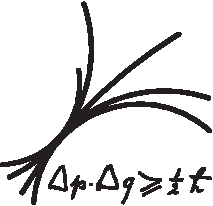
\includegraphics[width=0.15\textwidth]{logoMPPMU}\hfil
  \begin{minipage}[b]{0.5\linewidth}\centering
    \rule[-4.2mm]{\textwidth}{0.3mm}\\\rule{0.98\textwidth}{0.1mm}\\
    GERDA Scientific/Technical Report Munich\\\vspace{2mm}
    GSTR-09-M010 \\\vspace{2mm}
    Created: Sep. 04, 2009\\\vspace{-7.5mm}
    \rule[-5mm]{0.98\textwidth}{0.1mm}\\\rule{\textwidth}{0.3mm}\\
  \end{minipage}\hfil
  
\includegraphics[width=0.15\textwidth]{logoGERDA}%
\end{figure}

\begin{flushright}
Last updated: Sep. 04, 2009
\end{flushright}
\vspace{0.5cm}

\Large{Internal Note}
\vspace{1cm}

\LARGE{Dielectric Constant of Germanium}
\vspace{1cm}

\Large{Bonnie Chow$^{\dagger}$}
\vspace{0.5cm} 

\normalsize{$^{\dagger}$\textit{Max-Planck-Institut f\"ur Physik in M\"unchen}}
\vspace{0.5cm} 

\rule{0.9\textwidth}{0.1mm}
\begin{abstract}
 An attempt was made to measure the dielectric constant of germanium in liquid 
 nitrogen at high voltage, using a simple parallel-plate capacitor setup. For 
 electrical grade germanium in liquid nitrogen it was observed that the 
 resistivity is still too low for this method to be feasible, as the behaviour 
 is simply that of a conductor. Alternative methods are required to  determine 
 the dielectric constant of germanium.
\end{abstract}
\rule{0.9\textwidth}{0.1mm}

\end{titlepage} 


\section{Introduction}
\label{s:intro}

%such as in the calculation of various parameters or the design of capacitors.

The dielectric constant of a material is an important parameter of a material. Although it is described as a 'constant', it is actually dependent on temperature\textsuperscript{\cite{benedict91}-\cite{fukuroi}}, frequency and the strength of the applied electric field, amongst other conditions. We are especially interested in the dielectric constant of germanium at low temperatures and high electric field, since it is under these conditions which all Ge detectors are operated. The GERDA experiment\textsuperscript{\cite{gerda}}, searching for neutrinoless double beta decay in \textsuperscript{76}Ge, will use high-purity Ge detectors operating in cryogenic liquid. In order to simulate the pulse-formation inside the detector, it is necessary to calculate the electric field within. This can be done using

\begin{equation}
	\label{e:poisson}
	\nabla\cdot\textbf{E} = \frac{\rho}{\varepsilon_{0}\varepsilon_{r}}
\end{equation}
where \textbf{E} is the electric field, $\rho$ is the charge density, $\varepsilon_{0}$ is the permittivity of free space and $\varepsilon_{r}$ is the dielectric constant. The dielectric constant itself is defined as

\begin{equation}
	\label{e:def}
	\varepsilon_{r} = \frac{\varepsilon}{\varepsilon_{0}}
\end{equation}
where $\varepsilon$ is the permittivity of the material. Knowledge of $\varepsilon_{r}$ will also provide information on the electronic properties of Ge, which will be helpful in the design of readout systems from such detectors.

%equ in intro??



\section{Theoretical Model}
\label{s:theoretical}

Semiconductors have properties in between that of conductors and insulators. Inside a conductor, both bound and free charge are present. The electric field $E = 0$ within a conductor and so it cannot be electrically polarised. An insulator (dielectric) in contrast has bound charge only and is polarizable, as a result of the creation of electric dipoles within the material.

Conduction in a semiconductor such as Ge can be modelled by the movement of electrons and holes, which are positively charged states in the absence of an electron and is strongly temperature dependent. As the temperature increases, the resistivity of the semiconductor decreases since there are more electron-hole pairs due to thermal excitation. 

Under certain conditions, if the properties of the Ge sample are closer to that of an insulator, it will be possible then to measure the capacitance of the sample using a parallel-plate capacitor setup and hence calculate the $\varepsilon_{r}$. This can be done by applying the equation 
\begin{equation}
	\label{e:capacitor}
 	C = \varepsilon_{0}\varepsilon_{r}\frac{A}{d}
\end{equation}
where $C$ is the capacitance, $A$ is the area of the capacitor plates and $d$ is the distance between the plates. Published data on the room temperature dielectric constant of Ge include that of Benedict and Shockley$^{\cite{benedict89}}$ who found a value of 16.0$\pm$0.5 using a wave-guide method. Goldey and Brown$^{\cite{goldey98}}$ give two values, 16.4$\pm$0.2 and 16.6$\pm$0.3 using a similar technique as in \cite{benedict89} at 24GHz.
\\
If more than one material is present between the plates, the setup can be treated as several capacitors in series with each other and the following equation can be used:
\begin{equation}
 	\label{e:series}
	\frac{1}{C_{total}} = \frac{1}{C_{1}} + \frac{1}{C_{2}} + \cdots
\end{equation}

%In our experiment, we will insulate the Ge sample by placing it in between two isolation layers. The whole sample can then be treated as three capacitors in series.

%A value of 16.0$\pm$10\% was also made by Dacey$^{\cite{dacey90}}$. THIS WAS AT 77K
%put method which they used?



\section{Experimental Setup}
\label{s:expSetup}
To determine $\varepsilon_{r}$, a parallel plate capacitor was constructed using two circular Cu plates of diameter 67.25mm and thickness 1mm. A circular Ge sample of diameter 67.25mm and thickness 0.5mm was placed in between the plates, with an insulating layer of 0.05mm Kapton\textsuperscript{\copyright} film on both sides of the sample (Fig.2). 
The Ge sample is of electrical grade, 99.9999\% purity. Wires were soldered onto the Cu plates to provide electrical connections and the whole setup was then secured with Kapton\textsuperscript{\copyright} tape to prevent changes in $d$ during the experiment (Fig.1). A symmetrical arrangement was chosen so that the polarity of the power source would not have an effect on the measurements. The Cu plates were cleaned with acetone and a cleaning solution suitable for circuit components, to remove grease or oxide layers which may affect the results. Cu plates of 1mm thickness were chosen over thinner samples, as they will deform less through use, especially after being placed into LN$_{2}$.


\begin{figure}[htpb]
\centering
	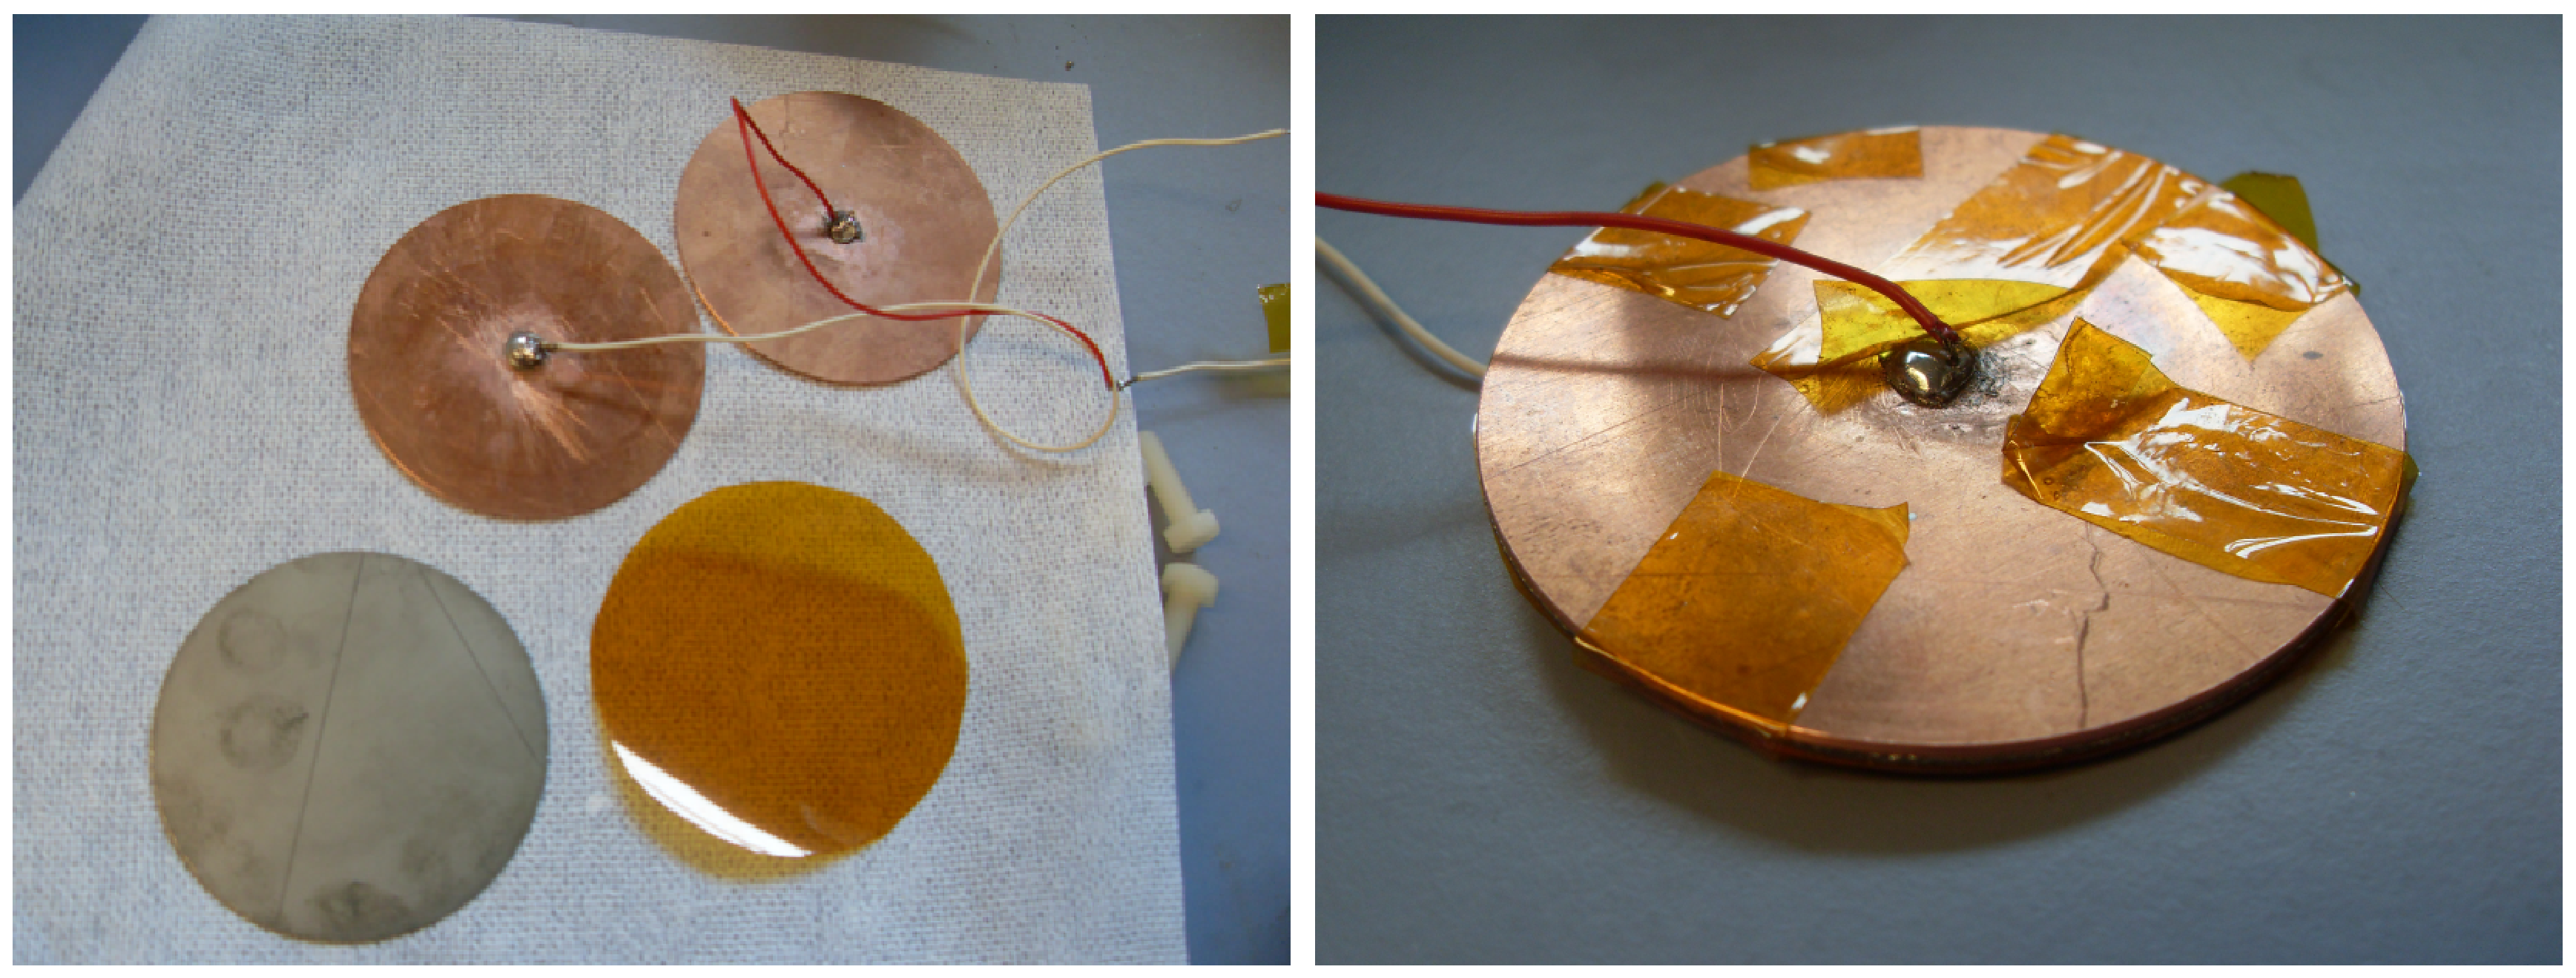
\includegraphics[scale=0.25]{sample_layer}
	\label{f:photosample}
	\caption{Showing the separate layers of Ge, Kapton\textsuperscript{\copyright} film and Cu plates. The image on the right is that of the assembled setup, secured with Kapton\textsuperscript{\copyright} tape.}
	
	%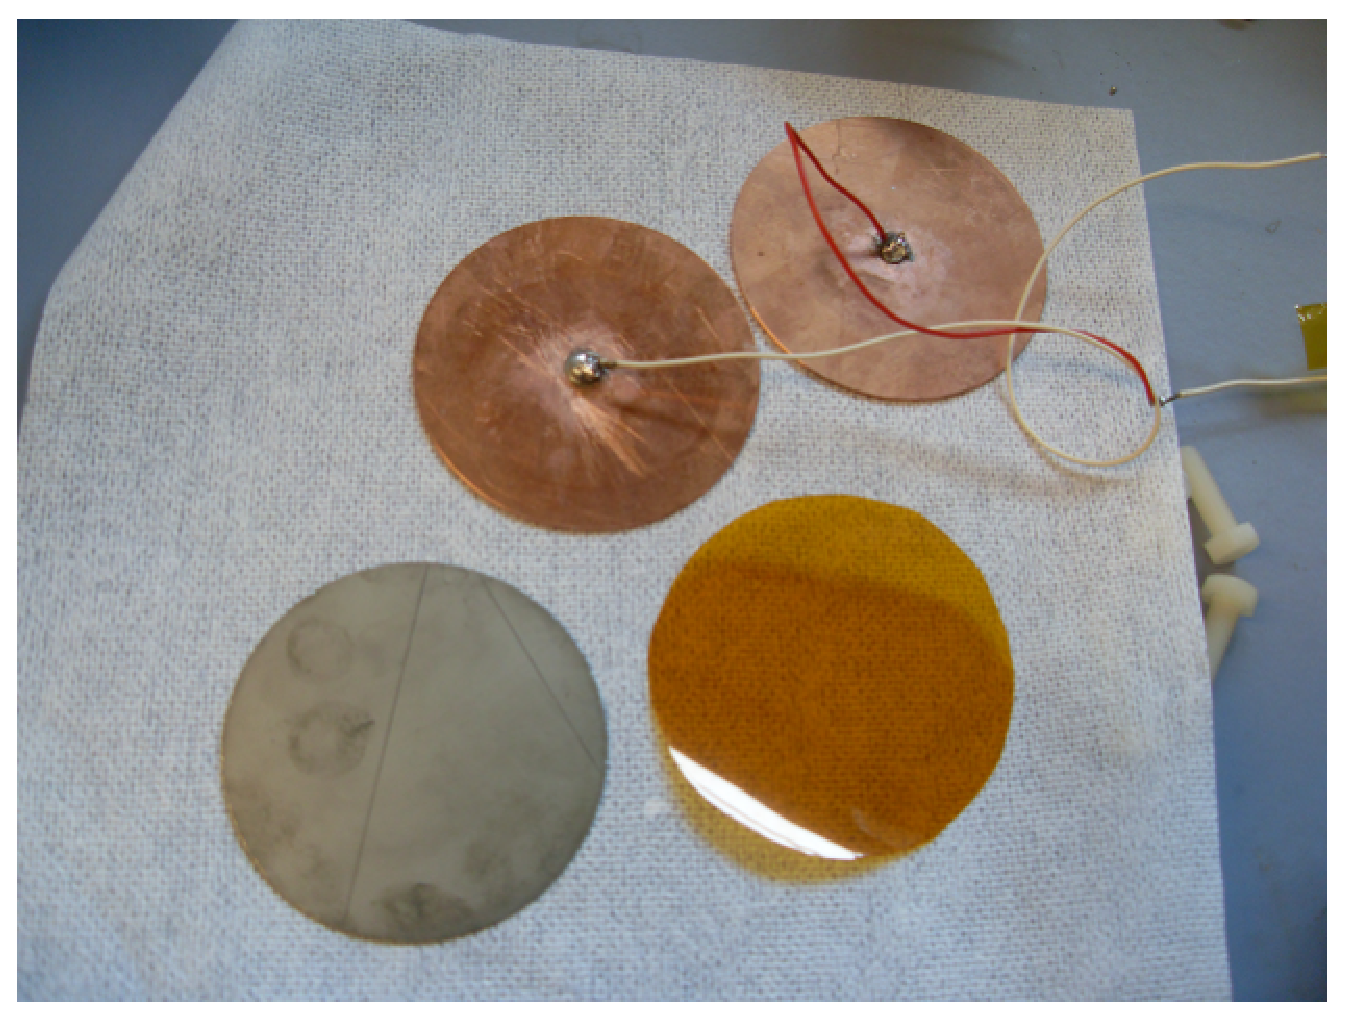
\includegraphics[scale=0.3]{layers}
	%\label{f:layers}
	%\caption{Showing the separate layers of Ge, Kapton\textsuperscript{\copyright} film and Cu plates.}
\end{figure}

\begin{figure}[htpb]
\centering
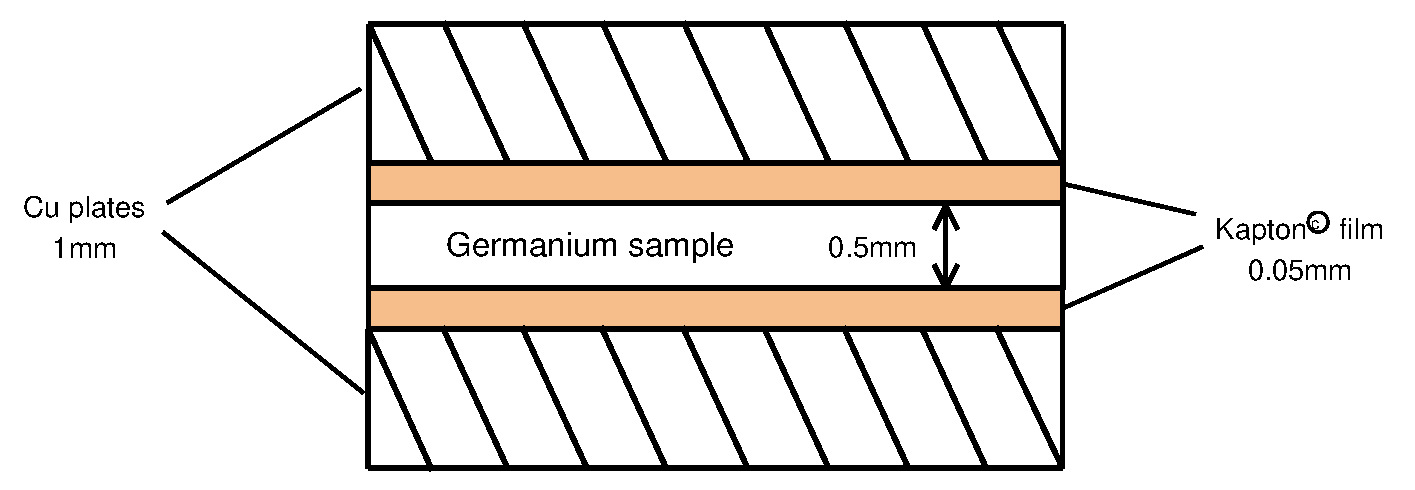
\includegraphics[scale=0.5]{crossSection}	
	\label{f:xsec}
	\caption{Cross section of sample setup with Kapton\textsuperscript{\copyright} film as the insulating layer}
\end{figure}


A Hewlett-Packard 4284A LCR meter was used during this measurement to measure the parallel capacitance $C_{p}$, the parallel resistance $R_{p}$, the series capacitance $C_{s}$ and the series resistance $R_{s}$ (see Fig.~\ref{f:setup}). These values were all recorded so more information about the arrangement of the circuit could be obtained. The relative sizes of $R_{p}$, $R_{s}$ will determine the simplifications to the general model (Fig.~\ref{f:setup}) which the LCR meter makes. If $R_{p} >> R_{s}$ then this indicates that our sample is closer to an ideal capacitor. A high voltage (HV) messbox, provided by Canberra France, was used in conjunction with the LCR meter to protect it from large currents when high voltages were applied.

\begin{figure}[htpb]
\centering
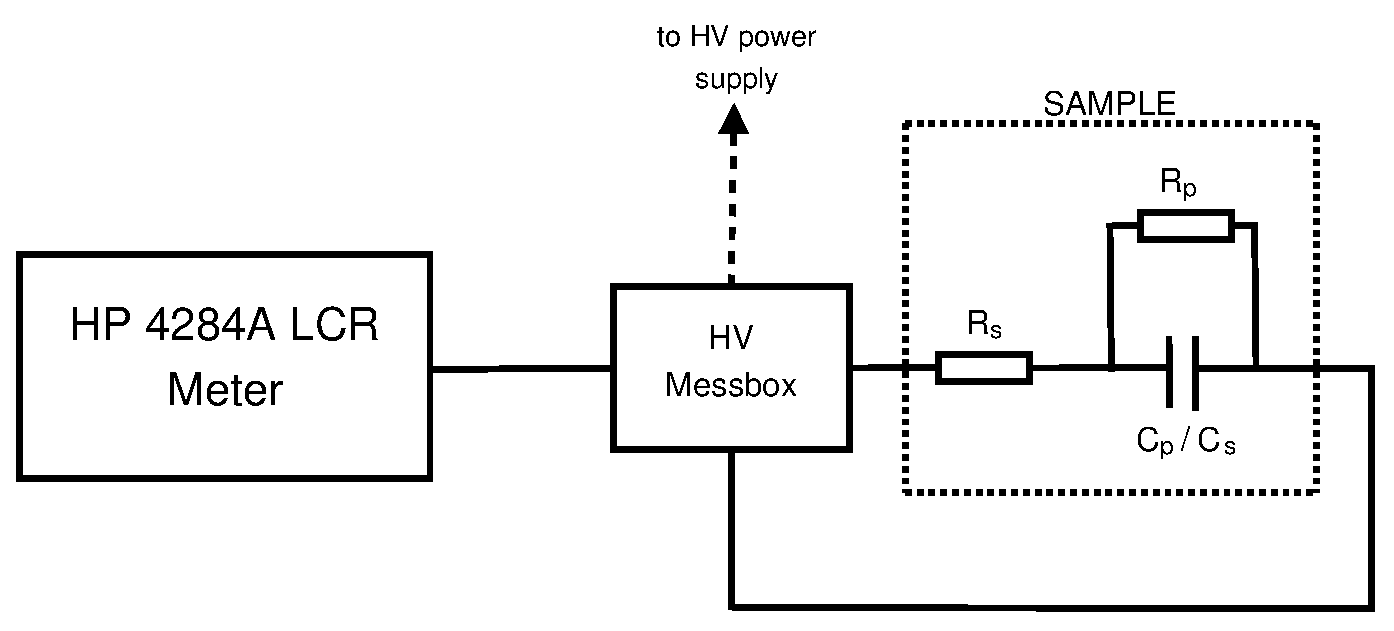
\includegraphics[scale=0.45]{basicsetup}
	\label{f:setup}
	\caption{Diagram of setup used. The sample under measurement is represented as a number of resistors and capacitors.}
\end{figure}



\section{Measurements}
\label{s:meas}

Measurements were first made at room temperature, starting at 0V and increasing in 100V increments until 600V , for frequencies from 100Hz to 1MHz. This voltage range was chosen because the maximum voltage gradient which will be present in the GERDA detectors are 300V/mm and hence for our 0.5mm sample we only require data up to 600V. The whole process was then repeated again with the sample setup placed inside a dewar filled with LN$_{2}$, cooling the sample to 77K. We measured at the highest frequency possible with this LCR meter, at 1MHz. This is because at low frequencies, we found that correct values for $R_{p}$, $R_{s}$ could not be obtained. For all the different materials examined, the $C_{p}$ and $C_{s}$ measured were identical up to three or four significant figures and so from here on, no distinction between the two will be made.\\
%why not obtained....``simplications fail??'' vague..

We found that there was essentially no variation with voltage as the maximum difference in capacitances measured was of the order of a few pF. An increase in capacitance of 40pF is observed when the sample is placed in L$N_{2}$. At both temperatures $R_{p}$ is much larger than $R_{s}$, suggesting that our setup is a good approximation of an ideal capacitor.

\begin{table}[htbp]
\label{t:KapGeRT}
\begin{center}
	\caption{Data for the Ge sample between two layers of Kapton\textsuperscript{\copyright} film, at 1MHz and room temperature.}
\begin{tabular}{| c | c | c | c | c |}
	\hline
	\multicolumn{5}{|c|}{At room temperature}\\
	\hline
		V/V & $C_{p}$/pF & $R_{p}$/k$\Omega$ & $C_{s}$/pF & $R_{s}$/$\Omega$\\ \hline
		
		0 & 271.53 $\pm$0.01 & 140.00 $\pm$0.05 & 271.48 $\pm$0.01 & 2.49 $\pm$0.02\\ \hline
		100 & 271.29 $\pm$0.01 & 118.85 $\pm$0.05 & 271.34 $\pm$0.01 & 2.87 $\pm$0.01\\ \hline
		200 & 271.51 $\pm$0.01 & 106.70 $\pm$0.05 & 271.49 $\pm$0.01 & 3.23 $\pm$0.01\\ \hline
		300 & 271.70 $\pm$0.02 & 98.40 $\pm$0.05 & 271.74 $\pm$0.01 & 3.48 $\pm$0.01\\ \hline
		400 & 272.03 $\pm$0.01 & 92.50 $\pm$0.05 & 272.02 $\pm$0.01 & 3.69 $\pm$0.02\\ \hline
		500 & 272.38 $\pm$0.01 & 87.72 $\pm$0.02 & 272.41 $\pm$0.01 & 3.90 $\pm$0.01\\ \hline
		600 & 272.86 $\pm$0.01 & 83.10 $\pm$0.05 & 272.86 $\pm$0.01 & 4.09 $\pm$0.01 \\
	\hline
\end{tabular}
\end{center}	
\end{table}


\begin{table}[htbp]
\label{t:KapGeLN2}
\begin{center}
	\caption{Data for the Ge sample between two layers of Kapton\textsuperscript{\copyright} film, at 1MHz in LN$_{2}$}
\begin{tabular}{| c | c | c | c | c |}
	\hline
	\multicolumn{5}{|c|}{In LN$_{2}$}\\
	\hline
		V/V & $C_{p}$/pF & $R_{p}$/k$\Omega$ & $C_{s}$/pF & $R_{s}$/$\Omega$\\ \hline
		
		0 & 309.964 $\pm$0.002 & 90.7 $\pm$0.1 & 309.980 $\pm$0.005 & 2.92 $\pm$0.01\\ \hline
		100 & 310.075 $\pm$0.005 & 95.4 $\pm$0.2 & 310.080 $\pm$0.005 & 2.75 $\pm$0.01\\ \hline
		200 & 310.382 $\pm$0.002 & 93.5 $\pm$0.1 & 310.394 $\pm$0.002 & 2.82 $\pm$0.01\\ \hline
		300 & 310.707 $\pm$0.005 & 91.1 $\pm$0.1 & 310.714 $\pm$0.002 & 2.87 $\pm$0.01\\ \hline
		400 & 310.980 $\pm$0.005 & 90.6 $\pm$0.1 & 311.002 $\pm$0.005 & 2.90 $\pm$0.01\\ \hline
		500 & 311.314 $\pm$0.005 & 87.9 $\pm$0.1 & 311.314 $\pm$0.005 & 2.96 $\pm$0.01\\ \hline
		600 & 311.700 $\pm$0.005 & 84.8 $\pm$0.1 & 311.720 $\pm$0.002 & 3.08 $\pm$0.01 \\
	\hline
\end{tabular}
\end{center}	
\end{table}

Using equations \ref{e:capacitor} and \ref{e:series}, the capacitance at 600V and given data$^{\cite{DuPont}}$ for the Kapton\textsuperscript{\copyright} film, we obtain a  $\varepsilon_{r}$ of 5.76 and 6.90 in room temperature and L$N_{2}$ respectively, both with errors of less than 0.005\%. Data from $\cite{DuPont}$ was taken to have no uncertainty and hence the only source of error here arises from the capacitance measurement. Our calculated value is inconsistent with the known room temperature $\varepsilon_{r}$ of Ge. 

We then focussed on other possible sources of uncertainty in our experiment. From \cite{DuPont}, it can be seen that $\varepsilon_{r}$ of Kapton\textsuperscript{\copyright} is almost constant with frequency, but varies greatly with temperature. To check the room temperature $\varepsilon_{r}$ and to compensate for the change to LN$_{2}$ temperature (77K), the capacitance of one layer of 0.05mm Kapton\textsuperscript{\copyright} film, $C_{Kap}$, was measured using the same setup. This process is described in section \ref{ss:kapOnly}.

\section{Systematic Uncertainty}
\label{s:sysUncertainty}

The distance between the Cu plates, $d$ is the largest source of uncertainty in this experiment. Earlier measurements were made, in which additional pressure was applied by securing the capacitor between polyethylene plates or using two ``C-clamps''. In this way we hoped to reduce the error in $d$ but it simple resulted in the Ge sample shattering when placed in LN$_{2}$. This was due to the slight deformation of the Cu and polyethylene plates. The effect of an increasing E-field on $d$ was considered by increasing the voltage to 600V and testing the amount of force required to pull the capacitor plates apart by hand. No extra effect was felt in comparison to zero voltage applied and hence there is no significant increase in pressure on the sample or variation in $d$ for voltages up to 600V. Hence it was both sufficient and necessary to use only Kapton\textsuperscript{\copyright} tape to secure the setup.

%hmmm...
The circuit itself provides extra capacitance $C_{circuit}$, observed by connecting the circuit without any device across it. In certain cases $C_{circuit}$ was much larger than the effect we wanted to measure.


\subsection{Measurements of Kapton$\textsuperscript{\copyright}$ only}
\label{ss:kapOnly}


\begin{table}[htbp]
\label{t:KapRT}
\begin{center}
	\caption{Data for one layer of Kapton\textsuperscript{\copyright} film, at 1MHz and room temperature.}
\begin{tabular}{| c | c | c | c | c |}
	\hline
	\multicolumn{5}{|c|}{At room temperature}\\
	\hline
		V/V & $C_{p}$/pF & $R_{p}$/k$\Omega$ & $C_{s}$/pF & $R_{s}$/$\Omega$\\ \hline
		
		0 & 388.14 $\pm$0.05 & 106.3 $\pm$0.4 & 388.08 $\pm$0.02 & 1.604 $\pm$0.002\\ \hline
		100 & 388.05 $\pm$0.01 & 89.5 $\pm$0.1 & 388.09 $\pm$0.01 & 1.871 $\pm$0.002\\ \hline
		200 & 388.59 $\pm$0.01 & 79.6 $\pm$0.1 & 388.57 $\pm$0.03 & 2.110 $\pm$0.005\\ \hline
		300 & 389.24 $\pm$0.01 & 73.4 $\pm$0.1 & 389.29 $\pm$0.01 & 2.279 $\pm$0.005\\ \hline
		400 & 390.03 $\pm$0.01 & 68.7 $\pm$0.1 & 390.01 $\pm$0.01 & 2.418 $\pm$0.005\\ \hline
		500 & 390.96 $\pm$0.01 & 65.1 $\pm$0.1 & 391.00 $\pm$0.01 & 2.551 $\pm$0.002\\ \hline
		600 & 392.21 $\pm$0.01 & 61.1 $\pm$0.1 & 392.21 $\pm$0.01 & 2.690 $\pm$0.001 \\
	\hline
\end{tabular}
\end{center}	
\end{table}


\begin{table}[htbp]
\label{t:KapLN2}
\begin{center}
	\caption{Data for one layer of Kapton\textsuperscript{\copyright} film, at 1MHz in LN$_{2}$.}
\begin{tabular}{| c | c | c | c | c |}
	\hline
	\multicolumn{5}{|c|}{In LN$_{2}$}\\
	\hline
		V/V & $C_{p}$/pF & $R_{p}$/k$\Omega$ & $C_{s}$/pF & $R_{s}$/$\Omega$\\ \hline
		
		0 & 466.020 $\pm$0.005 & 98.9 $\pm$0.1 & 466.050 $\pm$0.005 & 1.182 $\pm$0.002\\ \hline
		100 & 466.212 $\pm$0.005 & 92.2 $\pm$0.1 & 466.200 $\pm$0.005 & 1.260 $\pm$0.005\\ \hline
		200 & 466.780 $\pm$0.005 & 84.6 $\pm$0.2 & 466.800 $\pm$0.005 & 1.376 $\pm$0.002\\ \hline
		300 & 467.483 $\pm$0.005 & 78.2 $\pm$0.2 & 467.468 $\pm$0.005 & 1.474 $\pm$0.002\\ \hline
		400 & 468.230 $\pm$0.005 & 73.3 $\pm$0.1 & 468.280 $\pm$0.005 & 1.581 $\pm$0.003\\ \hline
		500 & 469.010 $\pm$0.005 & 68.7 $\pm$0.1 & 468.990 $\pm$0.005 & 1.670 $\pm$0.005\\ \hline
		600 & 469.950 $\pm$0.005 & 63.8 $\pm$0.1 & 469.990 $\pm$0.005 & 1.800 $\pm$0.005 \\
	\hline
\end{tabular}
\end{center}	
\end{table}


As before, there was only a tiny variation observed with voltage ($\approx$ 4pF). In room temperature, we expect $C_{Kap}$ $\approx$ 2.2nF, although a value of 392.21 $\pm$0.01pF was observed. If this $C_{Kap}$ is used instead of that obtained from \cite{DuPont} in equation \ref{e:series}, the capacitance of Ge, $C_{Ge}$, turns out to be negative. Likewise, in L$N_{2}$ the calculated $C_{Ge}$ is also negative.

By applying extra pressure with two ``C-clamps'' as shown in Fig. \ref{f:clamps}, one can alter the capacitance measured, with a maximum value of 1.1nF achieved. The large discrepancy between measured and expected values from the Kapton\textsuperscript{\copyright} film were attributed to uncertainty from $d$. A thicker insulating layer was required to reduce the percentage uncertainty in $d$. 

\begin{figure}[htpb]
\centering
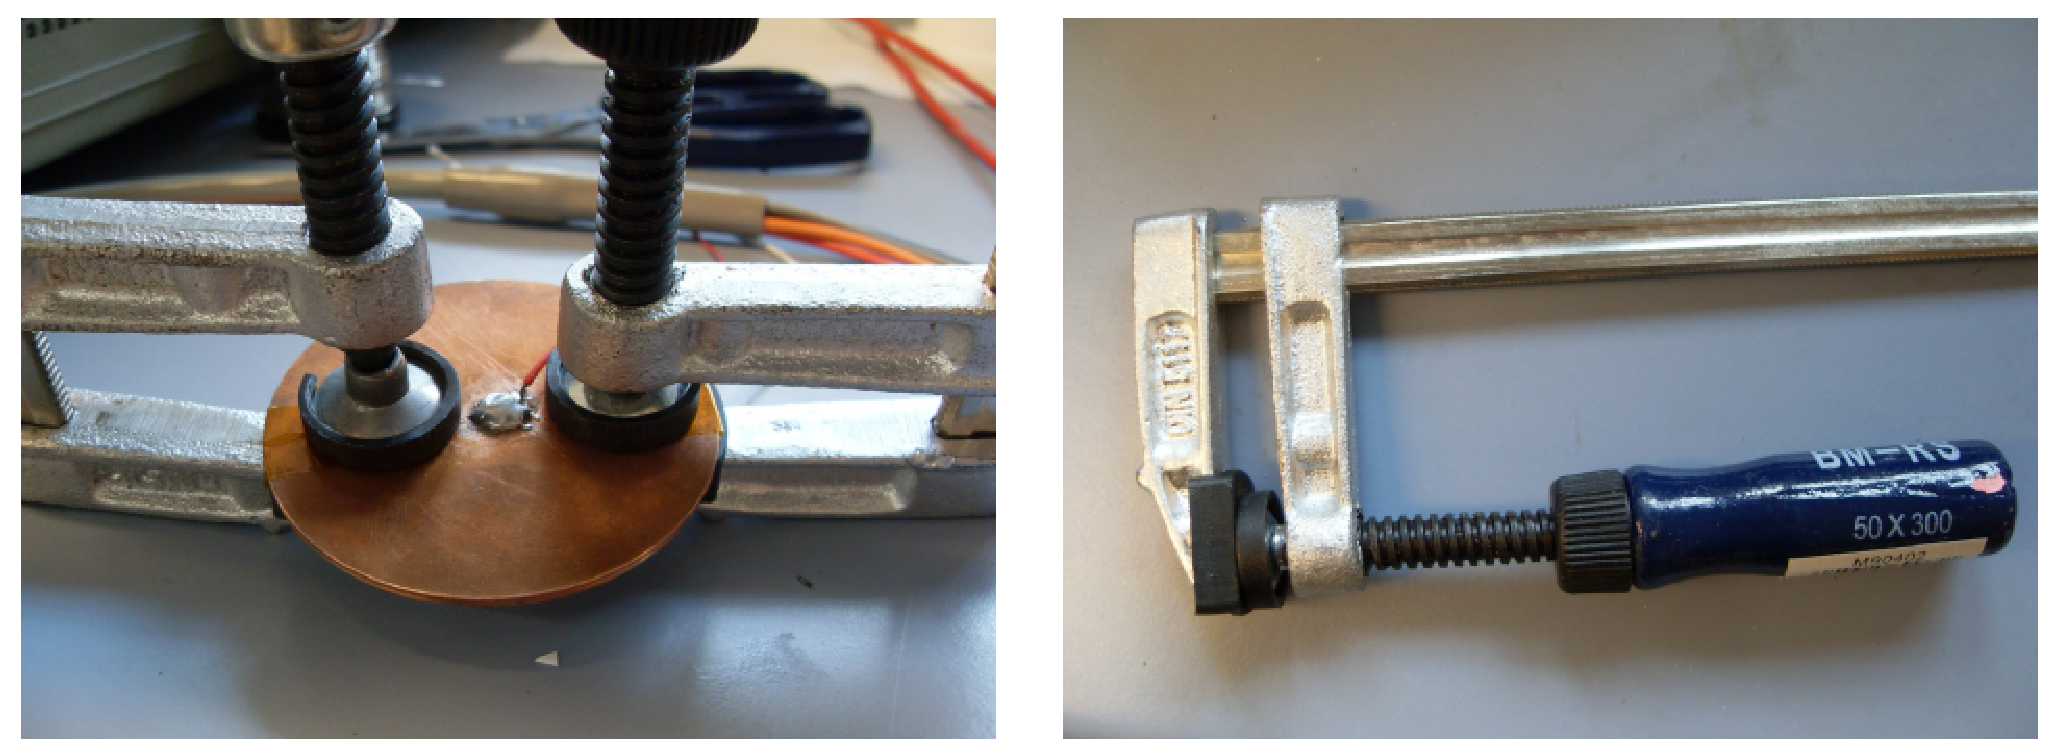
\includegraphics[scale=0.4]{clamps}
	\label{f:clamps}
	\caption{Showing the positioning of the C-clamps, as well as a side view of the clamp itself. The points of contact of the clamp are insulated from the sample.}
\end{figure}

\subsection{Measurements with Polyethylene}
\label{ss:PEonly}

10mm polyethylene samples were then chosen as the insulating layer between the Cu plates and the Ge sample, since the error in $d$ is much smaller in comparison and imperfections in the surface of the Cu plates were less significant. It also has a higher compressive strength than Kapton\textsuperscript{\copyright} film. With the Kapton\textsuperscript{\copyright} film, the error in $d$ was of the same order of magnitude as the thickness of the film itself, resulting in measurements of capacitance which was inconsistent with data from \cite{DuPont}.\\

Measuring with one layer of 10mm PE, the capacitance of PE, $C_{PE}$, at room temperature did not change significantly even when additional pressure was applied with ``C-clamps''. Again in both cases, no significant variation in capacitance with voltage was observed. Negative $R_{p}$, $R_{s}$ were observed when PE using as an insulating layer.\\

\begin{table}[htbp]
\label{t:polyRT}
\begin{center}
	\caption{Data for one layer of 10mm PE at 1MHz and room temperature.}
\begin{tabular}{| c | c | c | c | c |}
	\hline
	\multicolumn{5}{|c|}{At room temperature}\\
	\hline
		V/V & $C_{p}$/pF & $R_{p}$/M$\Omega$ & $C_{s}$/pF & $R_{s}$/$\Omega$\\ \hline
		
		0 & 8.8638 $\pm$0.0001 & -11.4 $\pm$0.1 & 8.8630 $\pm$0.0001 & -28.5 $\pm$0.2\\ \hline
		100 & 8.8662 $\pm$0.0001 & -12.2 $\pm$0.1 & 8.8666 $\pm$0.0001 & -25.8 $\pm$0.1\\ \hline
		200 & 8.8706 $\pm$0.0001 & -14.2 $\pm$0.1 & 8.8704 $\pm$0.0001 & -23.0 $\pm$0.1\\ \hline
		300 & 8.8737 $\pm$0.0001 & -15.7 $\pm$0.1 & 8.8737 $\pm$0.0001 & -20.3 $\pm$0.1\\ \hline
		400 & 8.8755 $\pm$0.0001 & -17.7 $\pm$0.1 & 8.8756 $\pm$0.0001 & -18.2 $\pm$0.1\\ \hline
		500 & 8.8762 $\pm$0.0001 & -19.8 $\pm$0.1 & 8.8761 $\pm$0.0001 & -16.2 $\pm$0.2\\ \hline
		600 & 8.8753 $\pm$0.0001 & -22.9 $\pm$0.1 & 8.8740 $\pm$0.0005 & -14.1 $\pm$0.1 \\
	\hline
\end{tabular}
\end{center}	
\end{table}


\begin{table}[htbp]
\label{t:polyLN2}
\begin{center}
	\caption{Data for one layer of 10mm PE, at 1MHz in LN$_{2}$.}
\begin{tabular}{| c | c | c | c | c |}
	\hline
	\multicolumn{5}{|c|}{In LN$_{2}$}\\
	\hline
		V/V & $C_{p}$/pF & $R_{p}$/k$\Omega$ & $C_{s}$/pF & $R_{s}$/$\Omega$\\ \hline
		
		0 & 10.200 $\pm$0.005 & -720 $\pm$10 & 10.200 $\pm$0.005 & -340 $\pm$5\\ \hline
		100 & 10.200 $\pm$0.005 & -720 $\pm$20 & 10.200 $\pm$0.005 & -330 $\pm$5\\ \hline
		200 & 10.202 $\pm$0.002 & -730 $\pm$10 & 10.207 $\pm$0.002 & -332 $\pm$5\\ \hline
		300 & 10.204 $\pm$0.005 & -740 $\pm$10 & 10.210 $\pm$0.005 & -330 $\pm$5\\ \hline
		400 & 10.204 $\pm$0.005 & -740 $\pm$20 & 10.208 $\pm$0.005 & -330 $\pm$5\\ \hline
		500 & 10.201 $\pm$0.005 & -740 $\pm$10 & 10.206 $\pm$0.005 & -329 $\pm$5\\ \hline
		600 & 10.200 $\pm$0.002 & -740 $\pm$10 & 10.206 $\pm$0.005 & -325 $\pm$5 \\
	\hline
\end{tabular}
\end{center}	
\end{table}


\begin{table}[htbp]
\label{t:polyGeRT}
\begin{center}
	\caption{Data for the Ge sample between two layers of 10mm PE at 1MHz, at room temperature.}
\begin{tabular}{| c | c | c | c | c |}
	\hline
	\multicolumn{5}{|c|}{At room temperature}\\
	\hline
		V/V & $C_{p}$/pF & $R_{p}$/M$\Omega$ & $C_{s}$/pF & $R_{s}$/$\Omega$\\ \hline
		
		0 & 4.7265 $\pm$0.0002 & -21.5 $\pm$0.2 & 4.7260 $\pm$0.0001 & -52 $\pm$1\\ \hline
		100 & 4.7262 $\pm$0.0002 & -23.2 $\pm$0.2 & 4.7264 $\pm$0.0002 & -49 $\pm$1\\ \hline
		200 & 4.7273 $\pm$0.0001 & -25.5 $\pm$0.3 & 4.7272 $\pm$0.0001 & -44 $\pm$1\\ \hline
		300 & 4.7281 $\pm$0.0001 & -28.0 $\pm$0.5 & 4.7283 $\pm$0.0002 & -39 $\pm$1\\ \hline
		400 & 4.7286 $\pm$0.0002 & -31.0 $\pm$0.5 & 4.7283 $\pm$0.0002 & -37 $\pm$1\\ \hline
		500 & 4.7279 $\pm$0.0001 & -33.0 $\pm$0.5 & 4.7282 $\pm$0.0002 & -33 $\pm$1\\ \hline
		600 & 4.7275 $\pm$0.0002 & -37.0 $\pm$0.5 & 4.7272 $\pm$0.0003 & -30 $\pm$1 \\
	\hline
\end{tabular}
\end{center}	
\end{table}

Using the $C_{tot}$ and $C_{PE}$ measured at 600V in room temperature, and equations \ref{e:capacitor} and \ref{e:series}, the $C_{Ge}$ calculated is still negative. Within the experimental error present, we cannot confirm the temperature dependence of the PE dielectric constant, although it must be a very small effect if it exists. As well as the large uncertainty present due to measuring such a small effect, the negative $C_{Ge}$ indicates that the resistivity of our sample is too low, even at 77K. This is discussed in more detail in section \ref{s:discuss}.

\subsection{Calibration Curve}
\label{ss:calib}

A systematic error due to the presence of the HV messbox was noticed. To correct for this a calibration curve was made by measuring the capacitance of a range of standard ceramic capacitors from up to 2nF, both with and without the messbox, at 1MHz with no external voltage applied. All values given below have now been corrected for the presence of the HV messbox. The errors on the corrected values are the same as that of the raw values, even after the calibration is taken into account, as they are very small in comparison to the measurements. 

%why 4.1 and not 4 for the figure??
\begin{figure}[htpb]
\centering
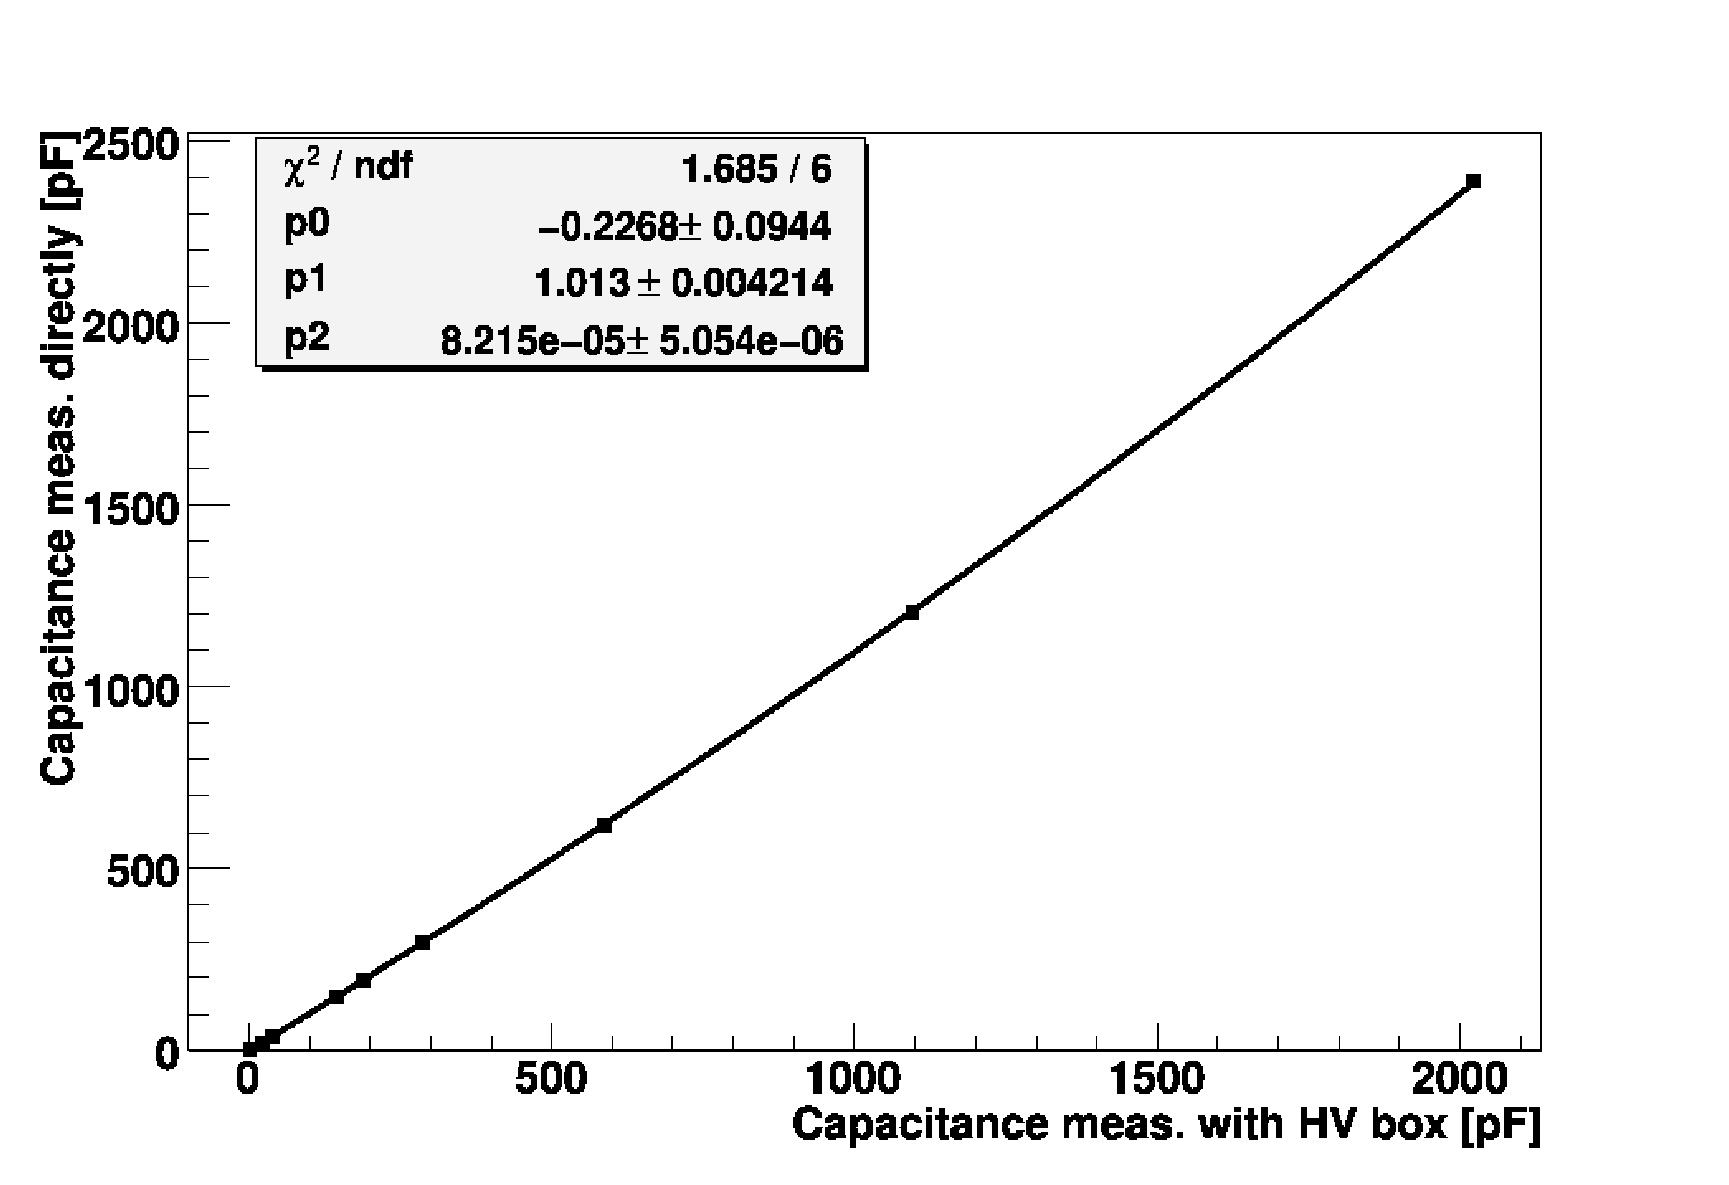
\includegraphics[scale=0.38]{calib}
	\label{f:calCurve}
	\caption{The calibration for 1MHz. The error bars are 1\% of the capacitance - approximately the error of the reading. A second order polynomial fit was applied to the data.}
\end{figure}


%sandwich data
\begin{table}[htbp]
\label{t:KapGec}
\begin{center}
	\caption{Corrected data for the Ge sample between two layers of Kapton\textsuperscript{\copyright} film at 1MHz.}
	
\begin{tabular}{| c | c | c |}
	\hline
	\multicolumn{3}{|c|}{At room temperature}\\
	\hline
		V/V & $C_{p}$/pF & $C_{s}$/pF\\ \hline
		
		0 & 280.95 $\pm$0.01 & 280.90 $\pm$0.01\\ \hline
		100 & 280.70 $\pm$0.01 & 280.75 $\pm$0.01\\ \hline
		200 & 280.93 $\pm$0.01 & 280.91 $\pm$0.01\\ \hline
		300 & 281.13 $\pm$0.02 & 281.17 $\pm$0.01\\ \hline
		400 & 281.48 $\pm$0.01 & 281.48 $\pm$0.01\\ \hline
		500 & 281.86 $\pm$0.01 & 281.88 $\pm$0.01\\ \hline
		600 & 282.36 $\pm$0.01 & 282.36 $\pm$0.01\\
	\hline
\end{tabular}
\hfill
\begin{tabular}{| c | c | c |}
	\hline
	\multicolumn{3}{|c|}{In LN$_{2}$}\\
	\hline
		V/V & $C_{p}$/pF & $C_{s}$/pF\\ \hline
		
		0 & 321.732 $\pm$0.002 & 321.750 $\pm$0.005\\ \hline
		100 & 321.850 $\pm$0.005 & 321.850 $\pm$0.005\\ \hline
		200 & 322.177 $\pm$0.002 & 322.190 $\pm$0.002\\ \hline
		300 & 322.523 $\pm$0.005 & 322.530 $\pm$0.002 \\ \hline
		400 & 322.810 $\pm$0.005 & 322.837 $\pm$0.005\\ \hline
		500 & 323.169 $\pm$0.005 & 323.169 $\pm$0.005 \\ \hline
		600 & 323.580 $\pm$0.005 & 323.601 $\pm$0.002\\
	\hline
\end{tabular}

\end{center}	
\end{table}


%kapton only
\begin{table}[htbp]
\label{t:KapRTc}
\begin{center}
	\caption{Corrected data for one layer of Kapton\textsuperscript{\copyright} film at 1MHz.}
\begin{tabular}{| c | c | c |}
	\hline
	\multicolumn{3}{|c|}{At room temperature}\\
	\hline
		V/V & $C_{p}$/pF & $C_{s}$/pF\\ \hline
		
		0 & 405.43 $\pm$0.05 & 405.36 $\pm$0.02\\ \hline
		100 & 405.33 $\pm$0.01 & 405.37 $\pm$0.01\\ \hline
		200 & 405.91 $\pm$0.01 & 405.89 $\pm$0.03\\ \hline
		300 & 406.61 $\pm$0.01 & 406.66 $\pm$0.01\\ \hline
		400 & 407.46 $\pm$0.01 & 407.44 $\pm$0.01\\ \hline
		500 & 408.46 $\pm$0.01 & 408.51 $\pm$0.01\\ \hline
		600 & 409.81 $\pm$0.01 & 409.81 $\pm$0.01\\
	\hline
\end{tabular}
	\hfill
\begin{tabular}{| c | c | c |}
	\hline
	\multicolumn{3}{|c|}{In LN$_{2}$}\\
	\hline
		V/V & $C_{p}$/pF & $C_{s}$/pF\\ \hline
		
		0 & 489.801 $\pm$0.005 & 489.830 $\pm$0.005 \\ \hline
		100 & 490.010 $\pm$0.005 & 490.000 $\pm$0.005 \\ \hline
		200 & 490.630 $\pm$0.005 & 490.650 $\pm$0.005\\ \hline
		300 & 491.396 $\pm$0.005 & 491.379 $\pm$0.005\\ \hline
		400 & 492.210 $\pm$0.005 & 492.265 $\pm$0.005 \\ \hline
		500 & 493.060 $\pm$0.005 & 493.039 $\pm$0.005\\ \hline
		600 & 494.090 $\pm$0.005 & 494.129 $\pm$0.005\\
	\hline
\end{tabular}
	
\end{center}	
\end{table}
	
	
%PE data
\begin{table}[htbp]
\label{t:polyRTc}
\begin{center}
	\caption{Corrected data for one layer of 10mm PE at 1MHz.}
\begin{tabular}{| c | c | c |}
	\hline
	\multicolumn{3}{|c|}{At room temperature}\\
	\hline
		V/V & $C_{p}$/pF & $C_{s}$/pF\\ \hline
		
		0 & 8.7607 $\pm$0.0001 & 8.7599 $\pm$0.0001\\ \hline
		100 & 8.7632 $\pm$0.0001 & 8.7636 $\pm$0.0001\\ \hline
		200 & 8.7676 $\pm$0.0001 & 8.7674 $\pm$0.0001\\ \hline
		300 & 8.7708 $\pm$0.0001 & 8.7708 $\pm$0.0001\\ \hline
		400 & 8.7726 $\pm$0.0001 & 8.7727 $\pm$0.0001\\ \hline
		500 & 8.7733 $\pm$0.0001 & 8.7732 $\pm$0.0001\\ \hline
		600 & 8.7724 $\pm$0.0001 & 8.7710 $\pm$0.0001\\
	\hline
\end{tabular}
\hfill
\begin{tabular}{| c | c | c |}
	\hline
	\multicolumn{3}{|c|}{In LN$_{2}$}\\
	\hline
		V/V & $C_{p}$/pF & $C_{s}$/pF\\ \hline

		0 & 10.117 $\pm$0.002 & 10.117 $\pm$0.005\\ \hline
		100 & 10.117 $\pm$0.005 & 10.117 $\pm$0.005\\ \hline
		200 & 10.119 $\pm$0.002 & 10.124 $\pm$0.002\\ \hline
		300 & 10.121 $\pm$0.005 & 10.127 $\pm$0.002\\ \hline
		400 & 10.120 $\pm$0.005 & 10.125 $\pm$0.005\\ \hline
		500 & 10.118 $\pm$0.005 & 10.123 $\pm$0.005\\ \hline
		600 & 10.120 $\pm$0.005 & 10.123 $\pm$0.002\\
	\hline
\end{tabular}

\end{center}	
\end{table}


\begin{table}[htbp]
\label{t:polyGeRTc}
\begin{center}
	\caption{Corrected data for the Ge sample between two layers of 10mm PE at 1MHz, at room temperature.}
\begin{tabular}{| c | c | c |}
	\hline
	\multicolumn{3}{|c|}{At room temperature}\\
	\hline
		V/V & $C_{p}$/pF & $C_{s}$/pF\\ \hline
		
		0 & 4.5641 $\pm$0.0002 & 4.5635 $\pm$0.0001\\ \hline
		100 & 4.5637 $\pm$0.0002 & 4.5639 $\pm$0.0002\\ \hline
		200 & 4.5649 $\pm$0.0001 & 4.5648 $\pm$0.0001\\ \hline
		300 & 4.5657 $\pm$0.0001 & 4.5659 $\pm$0.0002\\ \hline
		400 & 4.5662 $\pm$0.0002 & 4.5659 $\pm$0.0002\\ \hline
		500 & 4.5655 $\pm$0.0001 & 4.5658 $\pm$0.0002\\ \hline
		600 & 4.5651 $\pm$0.0002 & 4.5648 $\pm$0.0003\\
	\hline
\end{tabular}
\end{center}	
\end{table}

However even after the calibration, the $C_{Ge}$ calculated using Kapton\textsuperscript{\copyright} or polyethylene data are still negative.


\section{Discussion}
\label{s:discuss}

To test our model, the resistance of the Ge sample was measured and found to be of the order of a few ohms and tens of ohms, in room temperature and LN$_{2}$ respectively. %** compare with known resistivity values. Rs/Rp ?
It is incorrect to treat our setup as several capacitors in series, as the resistivity of electrical grade Ge is such that it acts as a conductor. Even in LN$_{2}$ when the resistance is an order of magnitude higher relative to room temperature, it is still too low to be regarded as a semiconductor. The current setup simply measures the capacitance of the insulating layers and in view of this it is unsurprising that it appears to be an ideal capacitor. With this procedure, we are unable to measure the dielectric constant of Ge.

		
\section{Alternative Methods}
\label{s:altMeth}

Instead of a parallel-plate capacitor, a diode could be constructed from our sample instead. This would allow the formation of a depletion zone within the Ge sample and hence an $E$-field. The capacitance of the diode could then be measured using the current apparatus and hence a $\varepsilon_{r}$ could be obtained. %define depletion zone??
\\
%One could also increase the resistivity of the Ge used by doping with a sufficient amount of gold leads. This method was used by Dunlap Jr. and Watters (**) ...also used parallel plate setup. 

Another alternative could be to use the resonant cavity method, as employed by Fukuroi and Yamagata$^{\cite{fukuroi}}$ to measure the dielectric constant of Ge at microwave frequencies. The impurities present in their Ge sample are estimated to be less than $10^{14}/cc$, much purer than our present sample. From 1.7 to 30K, $\varepsilon_{r}$ is found to be constant throughout this range, with a value close to 14.1 $\pm$0.3, depending on the geometry of the sample. At such low temperatures, there is insufficient energy for free charge carriers to be present within the Ge and it is plausible to infer that the only contribution to $\varepsilon_{r}$ is from the bound charge, the presence of which is independent of temperature. %no temp dependence? effective and relative??
Within their experiment, a large decrease in dielectric constant is observed in the temperature range 10-200K which is attributed to the temperature dependence of free charge carriers. This could have large implications for any experiment which uses the Ge dielectric constant since it has a significant temperature dependence.





\section{Conclusion}
\label{s:conc}

With our current setup, we cannot determine the dielectric constant of Ge at room temperature or L$N_{2}$. However, we have gained knowledge on the properties of Ge as well as other possible methods to determine the dielectric constant. Although the exact value of $\varepsilon_{r}$ for Kapton\textsuperscript{\copyright} film cannot be verified at these two temperatures, a temperature dependence can be seen. The temperature dependence of polyethylene cannot be confirmed as the changes are within experimental error.

\begin{thebibliography}{9} 
	\bibitem{gerda} http://www.mpi-hd.mpg.de/gerda/
	\bibitem{benedict91} T. S. Benedict, Phys. Rev. \emph{91}, 1565 (1953).
	\bibitem{benedict89} T. S. Benedict and W. Shockley, Phys. Rev. \emph{89}, 1152 (1953).	
	\bibitem{fukuroi} T. Fukuroi and K. Yamagata, 941st report, Research Institute for Iron, Steel and Other Metals.
	\bibitem{goldey98} J. M. Goldey and S. C. Brown, Phys. Rev. \emph{98}, 1761 (1955).
	\bibitem{dacey90} G. C. Dacey. Phys. Rev. \emph{90}, 759 (1953).
	\bibitem{DuPont} Summary of Properties for Kapton\textsuperscript{\copyright} Polyimide Films, DuPont{\begin{tiny}\texttrademark	                                                                                                                         \end{tiny}}.
\end{thebibliography}



\end{document}
